\chapter{The need for developments in uncertainty quantification}
In this chapter, we first motivate the need for stochastic models with a simple example predicting the path of a drifter in the Gulf Stream.
We then briefly review the current literature on stochastic parameterisation, which is the introduction of stochastic terms into otherwise deterministic models, in the context of atmospheric modelling, oceanography and climate forecasting.
Finally, we highlight the limitations of bulk stochastic simulation as a means of working with complicated stochastic models, both in terms of computational costs and accuracy.
This suggests the need, across a variety of applications, for developing computationally efficient methods for approximating prediction distributions of such stochastic models, which this thesis aims to address.



\section{Motivating example: the Gulf Stream}

To illustrate the importance of accounting for uncertainty when making predictions from an otherwise deterministic model, we shall provide a brief example that will be explored in more detail in \Cref{sec:appl_ocean}.

Suppose we are interested in tracking the position of a drifter on the surface of the ocean.
The only information we have available are measurements of the eastwards (zonal) and northwards (meridional) velocities at the surface, derived from altimetry (sea surface height) data.
Such data is available from the European Commission`s Copernicus Marine Environment Monitoring Service.

For the purposes of this example, assume that the position of the drifter at the initial time is known exactly\footnote{In practice, of course, this will not be the case, but this will introduce even more uncertainty into our model, furthering reinforcing the purpose of this example.}.
Assuming \td{need to check these assumptions! something}, the position \(x_t\) of the drifter on the surface at time \(t\) is the solution to
\[
	\dod{x_t}{t} = u\left(x_t, t\right),
\]
subject to the known initial position \(x_0\), where \(u\) is the appropriately interpolated surface velocity data.

\begin{figure}
	\begin{center}
		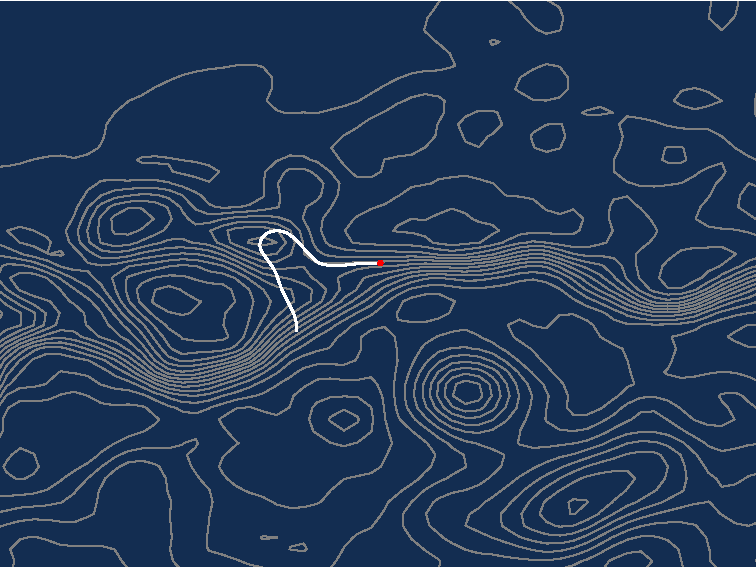
\includegraphics[width=\textwidth]{figures/gulf_stream_motivation/det_traj.pdf}
		\caption{The time evolution of the solution (obtained by numerically integrating the velocity data) to the deterministic system corresponding to \eqref{eqn:natl_sde}, from initial condition \(x_0 = \left(-60.5, 39\right)\) from 01/01/2021 (\(t = 0\)) to 08/01/2021 (\(t = 8\)).
			Contours of the sea surface height at the final time \(t = 8\) are included in grey to indicate the position of the Gulf Stream and nearby eddies in the flow.}
		\label{fig:na_motiv_det}
	\end{center}
\end{figure}

\Cref{fig:na_motiv_det} plots the resulting trajectory (in white) obtained by solving the deterministic position model numerically.

\begin{figure}
	\begin{center}
		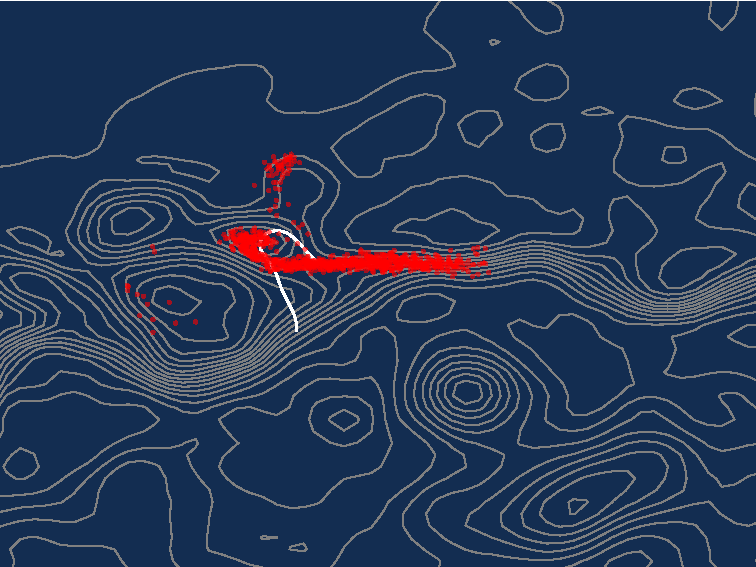
\includegraphics[width=\textwidth]{figures/gulf_stream_motivation/num_rels.pdf}
		\caption{The same visualisaton of the deterministic behaviour of the Gulf Stream example as \Cref{fig:na_motive_det}, but with the final positions of 10000 numerical realisations of a stochastic model, each indicated by a red point.}
		\label{fig:na_motiv_rels}
	\end{center}
\end{figure}



\Cref{fig:na_motiv_rels} shows us the result of numerically solving a stochastic differential equation formulation (specifically \eqref{eqn:natl_sde} in \Cref{sec:gulf_stream}) of the Lagrangian trajectory model.
This is a ``more correct'' model than the deterministic counterpart, in the sense that it is attempting to account for the unknowable measurement error and unresolved subgrid effects.
Each realisation here could correspond to our drifter, and we see a far different picture than the deterministic model alone provided.
Qualitatively, rather than following the Stream itself, a proportion of particles are caught in one of two eddies which have formed and broken off from the Stream.



Although deterministic models are often easier to work with analytically and far more efficient to solve numerically, these models are limited.






\section{Stochastic parameterisation in context}


The formal introduction of stochastic terms to account for unknown and unresolved processes into an otherwise deterministic model is known as \emph{stochastic parameterisation}, particularly in scientific circles.




The review by \citet{BernerEtAl_2017_StochasticParameterizationNew} summarises



Although stochastic parameterisation is more common in the atmospheric modelling context, it has also found emerging use in oceanography.

The mixing effect that these eddies have on the surrounding flow can be modelled with spatiotemporally-varying diffusion \citehere, which via the Fokker-Planck equation can be equivalently formulated as a stochastic differential equation with multiplicative noise.
The Lagrangian trajectories, incorporating these unresolved eddy effects, are then modelled as solutions to the stochastic differential equation.
Equivalently, through the Fokker-Planck equation we can consider the evolution of a passive tracer undergoing advection due to the deterministic drift and diffusion from both any natural diffusivity and the unresolved processes.
The probability density function that solves the Fokker-Planck equation can be instead thought of as a time-varying density (with the appropriate normalisation) of the tracer.
For instance, the Fokker-Planck equation has been used to model the transport of \citehere.
Hence, understanding the evolution of solutions to a stochastic differential equation is valuable in oceanography, as a means of quantifying both observational error and unresolved subgrid processes.


There are several different methods for quantifying eddy diffusivity given either observed tracer data or a global ocean circulation model.

The simplest notion of eddy diffusivity is a defined by






A recent approach by \cite{YingEtAl_2019_BayesianInferenceOcean} uses Bayesian inference to estimate the eddy diffusivity tensor from observed Lagrangian tracer data, by numerically solving the Fokker-Planck equation to compute a likelihood function.



% \section{Uncertainty quantification in Lagrangian coherent structures}
% As an alternative application,

% Lagrangian coherent structures are spatial regions within a flow that remain ``coherent'' in some sense over the evolution of the flow \citet{BalasuriyaEtAl_2018_GeneralizedLagrangianCoherent, AllshousePeacock_2015_LagrangianBasedMethods}.
% Standard examples include jet streams, eddies, and regions acting as barriers within the flow, but the idea of coherency
% For example, referring to our Gulf Stream

% There is an ongoing interest to understand the impact of Eulerian velocity uncertainty on coherent structures, and more generally on Lagrangian transport predictions \citep[e.g.]{Balasuriya_2020_StochasticApproachesLagrangian, Balasuriya_2020_UncertaintyFinitetimeLyapunov, BadzaEtAl_2023_HowSensitiveAre, BalasuriyaGottwald_2018_EstimatingStableUnstable, HallerEtAl_2018_MaterialBarriersDiffusive,BranickiUda_2021_LagrangianUncertaintyQuantification}.
% In particular, there is an emphasis on developing uncertainty quantification methods that are \emph{computational}, in the sense that they can be computed from only deterministic quantities of the system and do not rely upon stochastic simulation.
% Stochastic sensitivity, as introduced by \citet{Balasuriya_2020_StochasticSensitivityComputable}, fits into this interest, by providing one such computable measure, but by also introducing a novel approach for extracting coherent structures.
% Coherent regions, termed \emph{robust sets} by \citet{Balasuriya_2020_StochasticSensitivityComputable},



\section{Limitations of stochastic simulation}
The introduction of stochastic terms complicates both the analytical treatment of the model.
For example, we saw in \Cref{sec:sde_theory} that adding even additive and  stationary\lb{Is this the right word?? I mean that \(\sigma\) is constant, with no time-dependency}\td{need to define additive versus multiplicative properly.} noise to an analytically solvable non-linear deterministic model can make exact solutions intractable.
Thus, across many applications the state of the art approach is to generate samples of the stochastic model and perform statistical inference.
For example, Monte-Carlo simulation is used across weather forecasting \citep{LeutbecherEtAl_2017_StochasticRepresentationsModel}, \td{something atmospheric} and \td{something oceanic}.

However, the most significant drawback of bulk stochastic simulation is the computational load.
In general, a large number of samples is required for convergent statistics and accurate inference, as discussed by \citet{Leutbecher_2019_EnsembleSizeHow}.
For a complex model, the computational load of computing a single realisation

The recent review by \citet{LeutbecherEtAl_2017_StochasticRepresentationsModel} highlights the need to develop computationally efficient schemes for quantifying stochasticity in weather and climate forecast models.


\td{Show the plateauing out that I am observing empirically when using a KDE . . . some literature on this?? This is a huge point to make}
For example, suppose that we intend on using the probabilistic forecast of our stochastic model in an inference scheme, such as in data assimilation in which model predictions are combined with ongoing observations to produce an improved forecast \cite[e.g.]{LawEtAl_2015_DataAssimilationMathematical,BudhirajaEtAl_2019_AssimilatingDataModels, ReichCotter_2015_ProbabilisticForecastingBayesian}.
This requires a probability density function or similar for our forecast, but in generating samples we initially only have a collection of finite discrete points.


The overall aim of this thesis is to address this problem, by developing characterisations of uncertainty and algorithms for approximating solution probability densities (as opposed to just generating samples) that are computationally efficient.
We aim to take advantage of the computational ease of generating solutions to a deterministic system (relative to taking many samples of a stochastic one).


The purpose of this example was to highlight the importance of accounting for measurement error and unresolved processes in a ; when the dynamics are complicated, then any uncertainty can have a significant impact on our inferences from the model, both quantitatively and qualitatively.
